\section{Introduction}

%High Level Vision
Soft robots exhibit continuum body motion, large scale deformation, high compliance, and adjustable impedance  compared to traditional rigid-bodied robots with high impedance \cite{trivedi2008soft}. 
% whereas humans and animals have extremities with variable impedance.
%Soft robots won't necessarily replace existing rigid robot technologies, but complement it, because they can enable static and dynamic manipulations systems in nature are capable of.
%A further motivating factor for this work is that soft robots are inherently safer for interaction with humans and the environment due to their structural compliance and they can be lighter, one of the reasons why we research on that path.
%Fluidic robots have uses in scenarios where a classical robot would cause sparks and are dangerous. Why do we need accuracy if we have compliance. A 3DOF gripper is inherently not soft. A rigid gripper can not manipulate delicate objects without a lot of sensing.

Such characteristics make this class of robots well-suited for highly dexterous tasks and interactions that require conformation to environmental uncertainty.

Our goal is to develop a soft planar fluid-powered gripper and a motion planning algorithm that leverages a soft morphology to robustly grasp, drag, and place objects \dr{of unknown geometry}. 
%By utilizing softness in the design of our robot, we gain the ability to adapt to environmental variation \cite{mcmahan2006field}, harmlessly collide with the environment \cite{marchese2014whole}, and build resilience to unexpected external loads \cite{tolley2014resilient}; 
\rkk{In this paper we describe a planar soft robot manipulator we developed toward this goal.
We focus on the design, fabrication, control, and planning aspects of this soft robot.}

\begin{figure}[htb]
\centering
   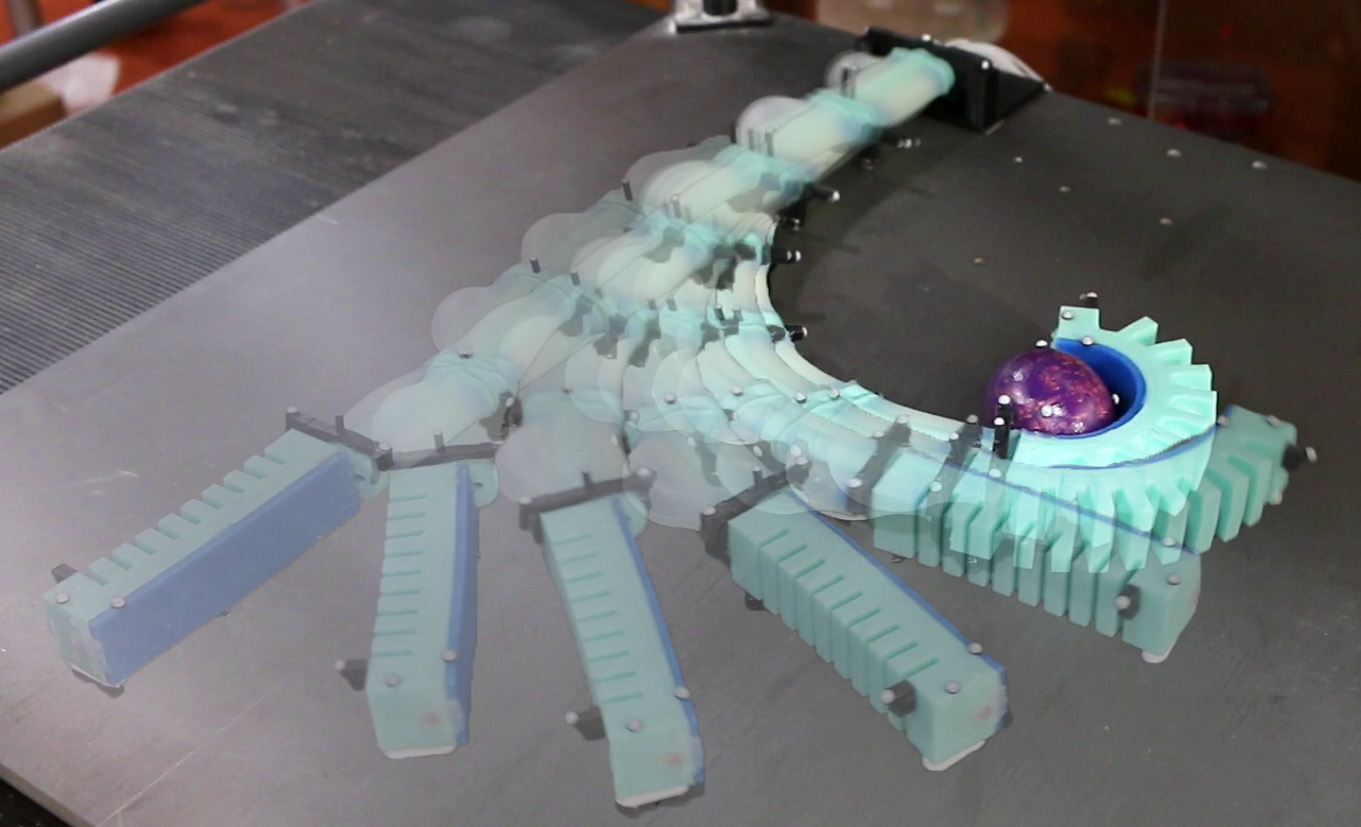
\includegraphics[width=0.99\columnwidth]{Figures/experimental_results/egg_approach/egg_approach_sequence_brighter}
   \caption{The soft manipulator is grasping an egg. The robot repeatably approached, grasped and moved this object.}
   \label{fig:egg_approach_sequence}
\end{figure}


%Challenges 
%Our manipulator is highly compliant and its motion is not as precise as more traditional rigid-bodied robots. 
%The control of its configuration is not only limited by the compliance of its low-pressure actuation, but also by its inherent elasticity.
%Additionally, the manipulator's compliant nature complicates the process of determining and sensing the forward kinematics.
%Despite the constraints on accurate positioning introduced by the softness of the arm, we can still robustly execute autonomous grasping tasks.

%\begin{figure}[htp]
%   \centering
%   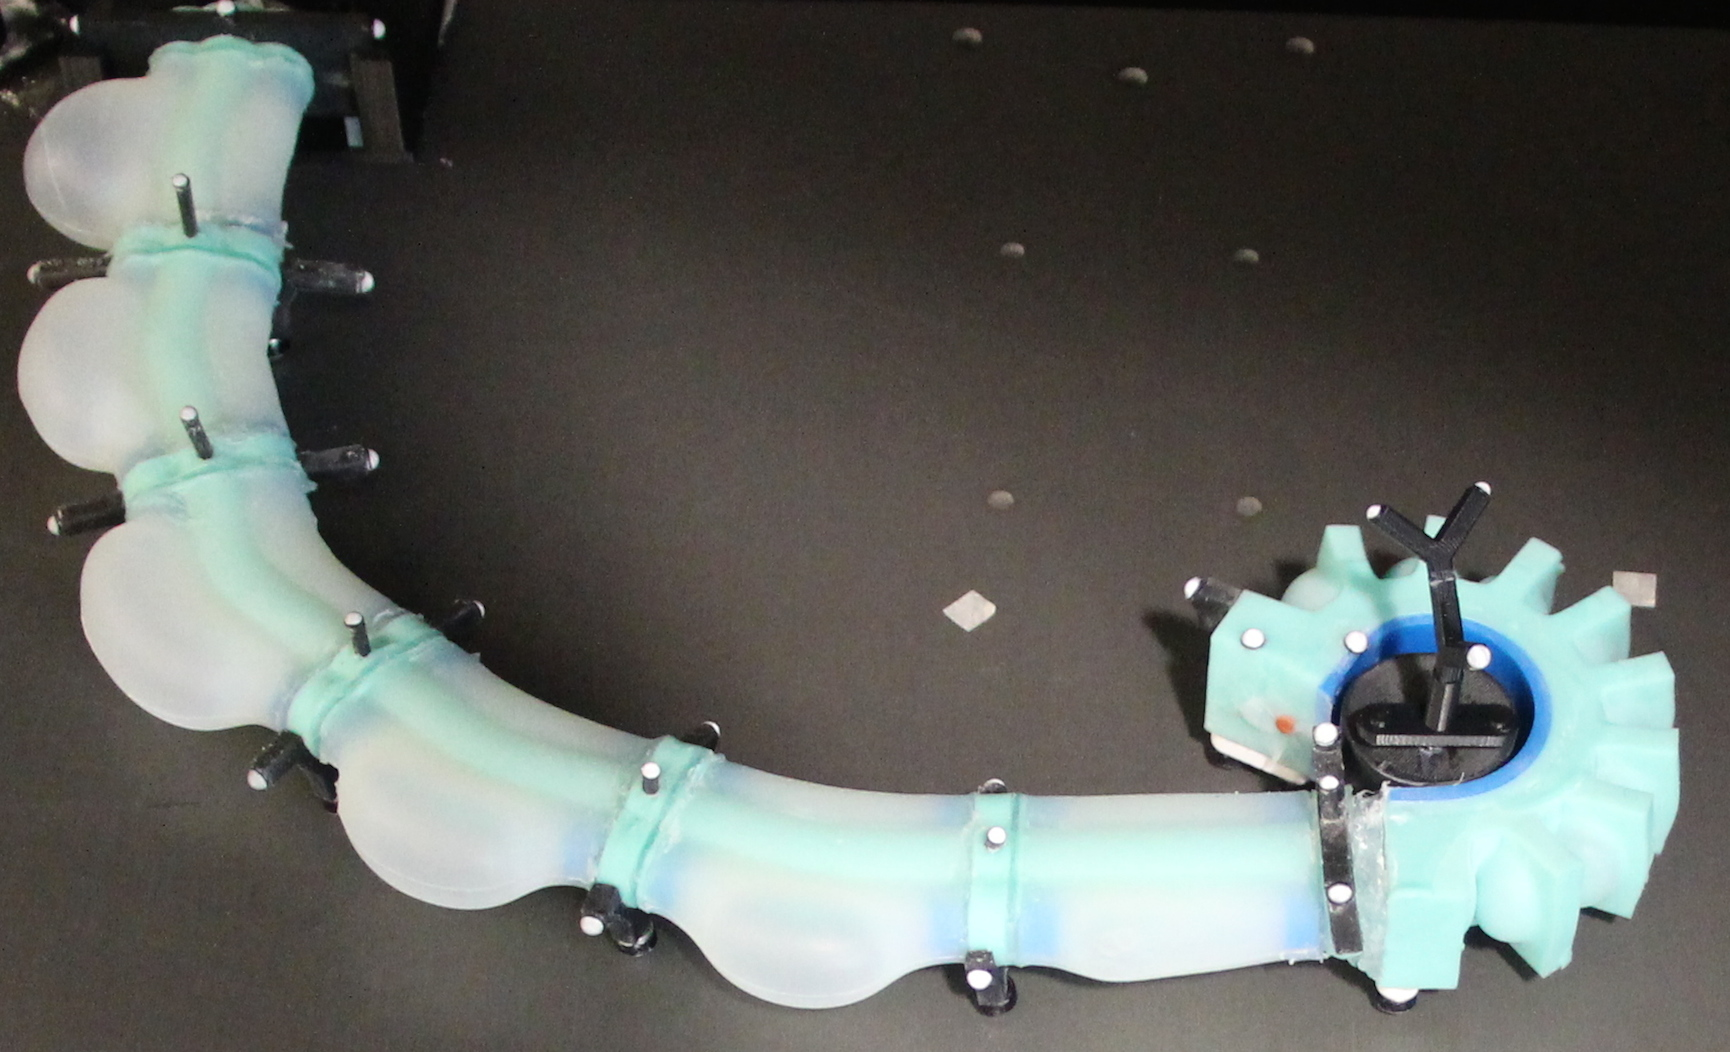
\includegraphics[width=0.7\columnwidth]{Figures/introduction/ExperimentalSetup}
%   \caption{A soft robotic arm with gripper autonomously approaching and grasping an object on a plane.}
%   \label{fig:intro}
%\end{figure}

%Our Approach
%To address these challenges, 
%We developed planning and control algorithms for a soft robotic arm with gripper.
The fluid-powered gripper at the end of the arm can grasp an object through an open-loop controlled bending motion, even if the gripper is positioned relatively inaccurately in relation to the object to be grasped.
%The gripper can conform due to his compliance to variations in object geometry, allowing it to successfully grasp.
The design of the gripper itself is inspired by the work of Polygerinos et al.~\cite{polygerinos2013towards}
The design is advantageous for grasping, because it exhibits high curvature, minimal radial expansion, and remains compliant during actuation. 
We can repeatably fabricate the gripper using a lost-wax casting process instead of the commonly used soft lithography technique.%, a multi-layer lamination process.
As a homogeneous piece without weakening seams, the gripper is not prone to de-lamination under high deformations. 
By abandoning the need for a lamination process, arbitrary shaped internal channels can be achieved. 

We attach the gripper to a multi-segment soft manipulator to enable autonomous grasp-and-place capabilities on a plane. 
Positional feedback is provided in real-time from a camera system.
%and actuation of the gripper and manipulator is driven by an external fluidic cylinder array.
\dr{Modeling uncertainties arise from a simplifying constant-curvature assumption, unrepresented manipulator dynamics, stick-slip friction, and non-linear fluidic control. 
These uncertainties are compensated by the inherent compliance of our soft gripper design and our motion planning strategy.}
The motion planning algorithm advances the arm through all the necessary states of the grasp-and-place operation.
A minimal strain, collision-free \dr{movement towards} the object of interest is found by posing the plan as a series of constrained nonlinear optimization problems.
The system first plans concentric approach circles shrinking from the initial end-effector pose down to the object diameter.
Next, the system searches for locally optimal manipulator configurations that constrain the end-effector to lie on these approach circles, so that the manipulator does not collide with the object. 
The manipulator is then moved between these plans using closed-loop trajectories. 
After successfully approaching the object, the gripper encapsulates it.
\dr{Even when the arm and gripper are fully actuated, they remain compliant allowing it to conform to un-modeled object geometries.}
We experimentally validate the system's ability to repeatably and autonomously grasp-and-place randomly placed objects.

\subsection{Related Work}
\dr{An overview of soft robotics is presented in Rus and Tolley \cite{rus2015design}. We will cover in the following the relevant works in fabrication, grippers and control of soft robots.}

Several manufacturing processes for soft biomimetic robots were reviewed by Cho et al. \cite{cho2009review}. 
The vast majority of soft elastomer robots rely on the processes of soft lithography \cite{xia1998soft} and/or shape deposition manufacturing \cite{cham2002fast}. 
Especially noteworthy is the use of wax for fabricating jammable skin chambers, which stiffens by vacuuming \cite{steltz2009soft}. 
The gripper presented in this work also uses a lost-wax molding technique, but with a different type of actuation in mind: the obtained cavity structures are inflated to cause the gripper to bend.

%\rkk{Volder et al. \cite{volder2010pneumatic} provides a detailed review of both pneumatic and hydraulic microactuators.} 
There are several hardware examples for soft grippers described in recent literature, we will mainly focus on fluidic-based systems.
Deimel and Brock \cite{deimel2013compliant} developed a pneumatically actuated three-fingered hand made of reinforced silicone that is mounted to a hard robot and capable of grasping.
More recently, they have developed an anthropomorphic soft pneumatic hand capable of dexterous grasps, which is not mounted to a robot, but instead held by a human \cite{deimel2014novel}. 
Using a soft-lithography fabrication, Ilievski et al. \cite{ilievski2011soft} created a pneumatic starfish-like gripper composed of an array of silicone chambers and a PDMS membrane. 
The gripper hangs on a string and grasps objects like an egg or a mouse in an open-loop controlled manner. 
Stokes et al. \cite{Stokes2014hybrid} use a soft elastomer quadrupedal robot attached to a wheeled robot to grip and retrieve objects. 
A puncture resistant soft pneumatic gripper is developed by Shepherd et al. in \cite{shepherd2013soft}. 
An alternative to positive pressure actuated soft grippers is a robotic gripper that makes use of granular material jamming developed by Brown et al. and detailed in \cite{brown2010universal}.
\rkk{Ikuta and Suzuki \cite{ikuta2002safety} demonstrated a multiple-segment micro-hydraulic actuator for entering blood vessels.}
The soft octopus-inspired arms developed in \cite{calisti2010study} and \cite{calisti2011octopus} are not fluidic powered, but instead use cables to pull rigid fixtures embedded within an elastomer body. 
The arms were capable of grasping objects like pens or screws.
A soft robotic tentacle developed in \cite{martinez2013robotic} was able to hold a flower and a horseshoe-shaped object.
The closest related soft pneumatic actuator design to our current work is the fast Pneu-net designs by Mosadegh et al. \cite{mosadegh2014pneumatic} and by Polygerinos et al. \cite{polygerinos2013towards}.
These finger-like actuators deform with minimal volume change and can bend to high curvatures.
None of the above described grippers were controlled autonomously to perform their tasks and accordingly no statement on repeatability of the autonomous execution was given. 

%talk about control
\rkk{Simulation results using an online motion planner for a planar continuum manipulators were presented by Xiao and Vatcha\cite{xiao2010realtime}.}
\rkk{This work was extended by Li and Xiao \cite{li2015general} to present a more general formulation to constrained, continuum manipulation.}
%More generally, the literature has several examples of soft pneumatic elastomer robots. 
%Many of these robots use open-loop controllers. 
%There are soft fluid-powered rolling robots \cite{correll2010soft, onal2011soft, marchese2011soft}. 
%Also, there are soft-bodied robotic fish powered by pneumatics \cite{marchese2014autonomous} and hydraulics \cite{katzschmann2014hydraulic}. 
%There are soft legged pneumatic walkers \cite{shepherd2011multigait, tolley2014resilient}, explosive jumpers \cite{shepherd2013using}, and 
Marchese et al. \cite{marchese2014design} demonstrated closed-loop position control of a multi-segment soft planar fluidic elastomer manipulator in free space. 
%Positioning is achieved using forward and inverse kinematic models and real-time camera measurements. 
%The manipulator curvatures are controlled in real-time using a curvature-volume cascaded control law.
\rkk{The soft manipulator presented in \cite{marchese2014whole} is only suitable for inspection tasks by moving through a constrained environment without object interaction or manipulation.}
%Previously, there were only single markers along the arm, which worked for a limited motion range, but was prone to fail if the markers go out of sight or another object is introduced to the environment. 
%Also, previously many trials were needed to successfully arrive at a final position.

\rkk{The work presented here combines two soft actuator types to leverage their strengths in a planar manipulation task. A new control method described here demonstrates the capabilities of this new soft manipulator to perform autonomous manipulations with uncertainties.}
%The control of the arm is improved from the previous version by using a more robust vision tracking approach. 

\subsection{Contributions}
We take on the challenge of grasping-and-placing objects with a seven degrees of freedom planar arm made entirely from soft rubber. 
Our work differs from the previous work in that we \rkk{create an entirely soft and autonomously controlled \emph{grasping} manipulation system.} 
\dr{Our planning and control method successfully copes with uncertainties in the object geometries, object placement and manipulator modeling.}
%We do not attach a novel soft gripper to a hard arm nor do we move the gripper around manually, 
We provide in this work the following contribution to soft robotics:
\begin{itemize}
  \item The design and fabrication process of a soft 2D manipulator.
  \item A planning algorithm to grasp-and-place randomly positioned objects on a planar surface using a 7 DOF soft manipulator.  
  \item \rkk{Autonomous manipulation experiments with various objects} \dr{of unknown geometry placed randomly in the working space of a soft manipulator} \rkk{without requiring force sensing or accurate positioning.} 
   \item Data from repeatable successful grasping demonstrations with a physical prototype and a \rkk{qualitative} experimental characterization of the uncertainty regions that can be tolerated by the soft gripper.
  %\item End-effector control of the grasping manipulator attached to a soft arm using a motion tracking system.
%\item A \rkk{controllable} soft manipulator consisting of a multi-segment arm with a gripper to enable fully compliant planar grasping.
\end{itemize}

%This paper is organized as follows: In Section~\ref{sec:System_Overview} we provide an overview of the planar manipulation system. In Section~\ref{sec:soft_grasping_manipulator} the gripper morphology is described, its operating principles are discussed in relation to existing morphologies, and the lost wax fabrication process is explained. Section~\ref{sec:processing_and_control} details the planning algorithms for grasp-and-place. Section~\ref{sec:experimental_results} shows results from experimental runs and provides evaluations and experimental insights. Lastly, Section~\ref{sec:conclusion} concludes by providing a summary and discussion.
